\documentclass[12pt,twoside]{article}
\usepackage{jmlda}
\usepackage{comment}
\usepackage{graphicx}

%\NOREVIEWERNOTES
\title
    [Определение местоположения по сигналам акселерометра] 
    {Определение местоположения по сигналам акселерометра}
\author
    [Зайнулина~Э.\,Т.] % список авторов для колонтитула; не нужен, если основной список влезает в колонтитул
    {Зайнулина~Э.\,Т., Киселёва~Е.\,А.,Фатеев~Д.\,А.,
    Божедомов~Н., Толканев~А.\,А., Ночевкин~В.,
    Протасов~В., Рябов~А.} % основной список авторов, выводимый в оглавление
    %[Автор~И.\,О.$^1$, Соавтор~И.\,О.$^2$, Фамилия~И.\,О.$^2$] % список авторов, выводимый в заголовок; не нужен, если он не отличается от основного
\thanks
    {
   Научный руководитель:  Стрижов~В.\,В.
    Консультант:  Мотренко~А.}
%\email
%    {zaynulina.et@phystech.edu}
%\organization
 %   {$^1$Московский физико-технический институт(ГУ)}
\abstract
    { {\textbf{Аннотация:}} данная статья посвящена методам отслеживания местоположения человека по сигналам акселерометра, гироскопа, магнитометра. Основной задачей исследования является увеличение точности позиционирования в условиях, когда глобальная навигационная система не может быть использована. В качестве базовой модели был выбран PDR (pedestrian dead reckoning). Для уменьшения зашумленности данных был использован фильтр Калмана. Новизна исследования заключается в постановке задачи в терминах Projection to Latent Spaces.

\bigskip
\textbf{Ключевые слова}: \emph {Pedestrian dead reckoning, (Indoor) inertial positioning, Simultaneous Localization and Mapping, PLS}.}

\begin{document}
\maketitle
%\linenumbers

\section{Введение}
В настоящее время системы по определению местоположения человека стали неотъемлемой частью повседневной жизни. Информация о точном местоположении человека используется для обеспечения безопасности, для ``мобильного здоровья'', для эффективной организации рабочих процессов, для мониторинга толпы и др. Огромную роль в определении местоположения человека играет GNSS (глобальная навигационная система). Однако в помещении навигационные спутниковые сигналы не всегда доступны, из-за чего качество данных, предоставляемых GNSS, сильно уменьшается. Тем не менее большую часть времени человек проводит в помещениях, в связи с чем должны быть разработаны надежные, точные методы, позволяющие определять местоположение человека в помещении.

Современные смартфоны обладают большим числом сенсоров и высокой вычислительной способностью. Так как в настоящее время почти каждый человек им обладает, то методы определения местоположения человека с использованием смартфонов получили наибольшее внимание со стороны исследователей. Среди этих методов - методы, основанные на беспроводных сигналах (WiFi, Bluetooth, UWB)\cite{journals/puc/VeraOA11}\cite{journals/puc/KimJP13}, датчиках обзора (лазерный сканер, монокулярная и бинокулярная камера)\cite{journals/puc/BrunsB09}, инерционных датчиках (акселерометр, гироскоп, магнитометр)\cite{journals/puc/ParkSC13}\cite{journals/puc/HardeggerRT15}\cite{journals/sensors/WangLYJG18}\cite{6987239}. Многие из предложенных методов локализации человека представляют собой комбинацию выше перечисленных для увеличения точности позиционирования\cite{journals/ejasp/EvennouM06}\cite{6834746}\cite{7021969}. Методы, основанные на беспроводных сигналах и датчиках обзора, помимо наличия смартфона требуют также введения дополнительного оборудования либо наличия дополнительных знаний, например карты помещения или базы данных силы сигнала (RSSI) WiFi точки в зависимости от координаты (WiFi fingerprint). Однако не всегда возможно предоставить карту помещения, например, в силу конфиденциальности; вспомогательное оборудование, в свою очередь, требует технического обслуживания и больших затрат. Что касается WiFi позиционирования, то при наличии существующей базы данных WiFi fingerprint при некотором изменении среды, позиционирование будет неточным, поэтому база данных нуждается в постоянном обновлении\cite{journals/sensors/Torres-Sospedra17a}.

Чтобы избежать данных проблем, предлагается метод, основанный на инерционных датчиках. В качестве базового алгоритма рассматривается pedestrian dead reckoning (PDR)~\cite{7743695}. По сравнению с методами, основанными на беспроводных сигналах и датчиках обзора, PDR рассчитывает относительно точное местоположение человека быстрее и потребляя меньше вычислительной мощности. Для фильтрации шума в данных используется фильтр Калмана~\cite{journals/corr/abs-1712-09004}. Особенность данной работы состоит в том, чтобы восстанавливать траекторию не от точки к точке, а всю целиком. Для работы с полученным многомерным пространством предлагается использовать метод PLS\cite{10.1007/11752790_2}.

\section{Постановка задачи}
Данные, полученные с помощью инерционных датчиков, представляют собой многомерные временные ряды $s(t) \in \mathbb{R}^N$. Каждому временному ряду сопоставляется вектор признаков. Эти вектора образуют матрицу признаков $X \in \mathbb{R}^{N \times T}$. По матрице $X$ необходимо предсказать траекторию пешехода $Y \in \mathbb{R}^{2 \times T}$, где строками матрицы $Y$ являются временные ряды $y(t)$, описывающие изменения глобальных координат (широта и долгота соответственно) пешехода во времени. Искомая модель:
\[f: X \to Y\]

В силу зависимости получаемых данных от расположения смартфона данная задача разбивается на 2 подзадачи. Первая подзадача состоит в том, чтобы определить класс $P$ расположения датчиков: нога, рука, сумка, тело ($\{0, 1, 2, 3\}$). Вторая подзадача состоит уже в предсказании траектории на основе полученного класса:
\[f \to f_1 ~ f_2\]
\[f_1: X \to P = \{0, 1, 2, 3\}\]
\[f_2: X, ~P \to Y\]

Для решения данных задач используется метод опорных векторов, который минимизирует следующий функционал $S(w|f, X, Y)$:

\[\min_{w, w_0}S(w, w_0) = \|w\|^2+C\sum_{i}\xi_i\]
\[subject~to~y_i(w^Tx_i+w_0)\geq 1-\xi_i~and~\xi_i \geq 0~\forall i\]

Для оценки качества модели используется критерий суммы квадратов отклонений предсказанных координат от истинных, а также корреляция между предсказанной и истинной траекториями пешехода.

\begin{comment}
Предполагается, что скорости, полученные в ходе решения данной задачи, содержат смещение $x^f_I$ ($I$ - система координат устройства), вызванное ошибками измерений датчиков. Относительно данного смещения делается предположение, что оно является низко-частотным. В результате решается следующая задача минимизации:
\[\min_{\{x^1_I, x^51_I,\dots\}}\sum_{f \in F_2}\|v_C^F-v_R^f\|+
\lambda\sum_{f \in F_1}\|x^f_I\|^2,\]
\[v_C^f = R_{SW}^f\sum_{f'=1}^f R_{WI}^{f'}(a_I^{f'}+x_I^{f'}),\]
где $f$ - единица блока выборки, $F$ - блок выборки, $v_C^F$ - скорректированное значение скорости, $v_R^f$ - предсказанное значение скорости, $W$ - глобальная система координат, $S$ - IMU-стабилизированная система координат, $R_{AB}$ - матрица перехода из системы координат $B$ в систему координат $A$.
\end{comment}


Формально постановку задачи можно записать следующим образом:
\[w^* = \arg\min_{w}S(w|f, X, Y).\]

\section{Базовый алгоритм}

Для получения матрицы признаков $X$ предварительно из данных удаляются высоко-частотные шумы с помощью сглаживания Гаусса. Полученные линейные и угловые скорости уже преобразуются в вектор признаков.

В качестве базового алгоритма используется каскадная регрессия, состоящая из SVM-классификатора и 8 SVR-регрессоров~\cite{journals/corr/abs-1712-09004}. 

По матрице признаков $X$ SVM-классификатор определяет, какому расположению датчиков (в руке, на ноге, на поясе, в сумке) соответствует данное описание, т.е. решает задачу многоклассовой классификации с 4 классами.

После этого для каждого класса на тренировочной выборке обучается свой SVR-регрессор, который выдает скорости движения пешехода для каждого временного блока. Полученные скорости содержат ошибку, связанную с неточностями инерционных датчиков, поэтому далее для этих скоростей находится смещение (по предположению низко-частотное) из следующей задачи минимизации:

\[\min_{\{x^1_I, x^51_I,\dots\}}V_{bias}=
\min_{\{x^1_I, x^51_I,\dots\}}\sum_{f \in F_2}\|v_C^F-v_R^f\|+
\lambda\sum_{f \in F_1}\|x^f_I\|^2,\]
\[v_C^f = R_{SW}^f\sum_{f'=1}^f R_{WI}^{f'}(a_I^{f'}+x_I^{f'}),\]
где $f$ - единица блока выборки, $F$ - блок выборки, $v_C^F$ - скорректированное значение скорости, $v_R^f$ - предсказанное значение скорости, $I$ - система координат устройства, $W$ - глобальная система координат, $S$ - IMU-стабилизированная система координат, $R_{AB}$ - матрица перехода из системы координат $B$ в систему координат $A$.

Также для каждого класса создается SVR-регрессор, предсказывающий угловые скорости пешехода в каждом временном блоке. 

На контрольной выборке для SVM-классификатора и каждого SVR-регрессора подбираются оптимальные значения гиперпараметров.

По полученным значениям скоростей восстанавливается траектория пешехода.

Формально алгоритм описывается следующим образом: 

После получения из данных матрицы признаков $X$

\begin{algorithmic}[1]
\REQUIRE $X, Y_{class}, Y, X_{test}$
\STATE $initialize ~ classifier\_options$
\STATE $classifier = SVMClassifier(classifier\_options);$
\STATE $classifier.fit(X, Y_{class})$
\FOR {$cls ~ in ~ classes$:}
\STATE $initialize ~ regressor\_cls\_optons$
\STATE $regressor\_cls = SVRRegressor(regressor\_cls\_optons)$
\STATE $regressor\_cls.fit(X[X[ind] \in cls], Y)[Y[ind] \in cls])$
\ENDFOR
\STATE $Y_{test-class} = classifier.predict(X_{test})$
\FOR {$cls ~ in ~ classes$:}
\STATE $Velocity\_cls = regressor\_cls.predict(X_{test}
[Velocity\_class[ind] == cls]$
\STATE $x^1_I, x^51_I,\dots = \argmin_{\{x^1_I, x^51_I,\dots\}}V_{bias}\_cls$
\STATE $Velocity\_cls = R_{SW}^f\sum_{f'=1}^f R_{WI}^{f'}(a_I^{f'}+x_I^{f'})$
\STATE $Trajectory\_cls$ recovery depending on $Velocity\_cls$
\ENDFOR
\RETURN $Full\_trajectory$
\end{algorithmic}

\section{Базовый эксперимент}

Цель эксперимента: найти параметры моделей такие, что предсказанная траектория пешехода будет наиболее близкой к истинной.

Для эксперимента используется часть данных, собранных в статье, описывающей алгоритм RIDI~\cite{journals/corr/abs-1712-09004}. Эти данные были получены с помощью инерционных датчиков, расположенных в смартфонах в нескольких случаях: когда смартфон располагался на поясе, в руке, на ноге или в сумке. Выборки содержат различные траектории длиной в 100 минут и частотой сигнала 200 Гц. В качестве объекта рассматривается положение в определенный момент времени $i$. Признаками объекта являются угловые скорости и линейные ускорения в стабилизированной системе координат датчиков в моменты времени $i-window\_size, \dots, i$, где $window\_size$ - размер окна (равен 200). Целевыми переменными являются метки классов, характеризующие то, в каком положении находился смартфон при получении определенных данных, а также скорости в данный момент времени $i$, которые вычисляются через координаты пешехода и прошедшее время. По полученным данным после уточнения скоростей с помощью оптимизации функции  $V_{bias}$ строится предсказанная траектория пешехода.

В ходе эксперимента исследовалась зависимость качества моделей на контрольной выборке в зависимости от параметров SVM-регрессоров.  Во всех моделях в качестве ядер были выбраны радиальные базисные функции, подбирались такие параметры как коэффициент штрафа $C$ и ядерный коэффициент $\gamma$. Качество измерялось с помощью кросс-валидации. Из результатов эксперимента следует, что для каждого расположения смартфона и каждого канала данных должны быть выбраны свои параметры модели.  Это подтверждает разумность классификации типа расположения смартфона перед непосредственным предсказанием траектории. 

Графики зависимости качества предсказания модели от параметров:

\begin{enumerate}
    \item Выборка 1 состоит из 30742 объектов (8728 объектов класса рука, 6106 объектов класса нога, 7758 объектов класса тело, 8150 объектов класса сумка).
    
    \item Выборка 2 состоит из 42731 объектов (13204 объектов класса рука, 8083 объектов класса нога, 11105 объектов класса тело, 10339 объектов класса сумка).
    
    \item Выборка 3 состоит из 35892 объектов (9458 объектов класса рука, 7304 объектов класса нога, 13306 объектов класса тело, 5824 объектов класса сумка).
    
\end{enumerate}
    
    \begin{figure}[H]
    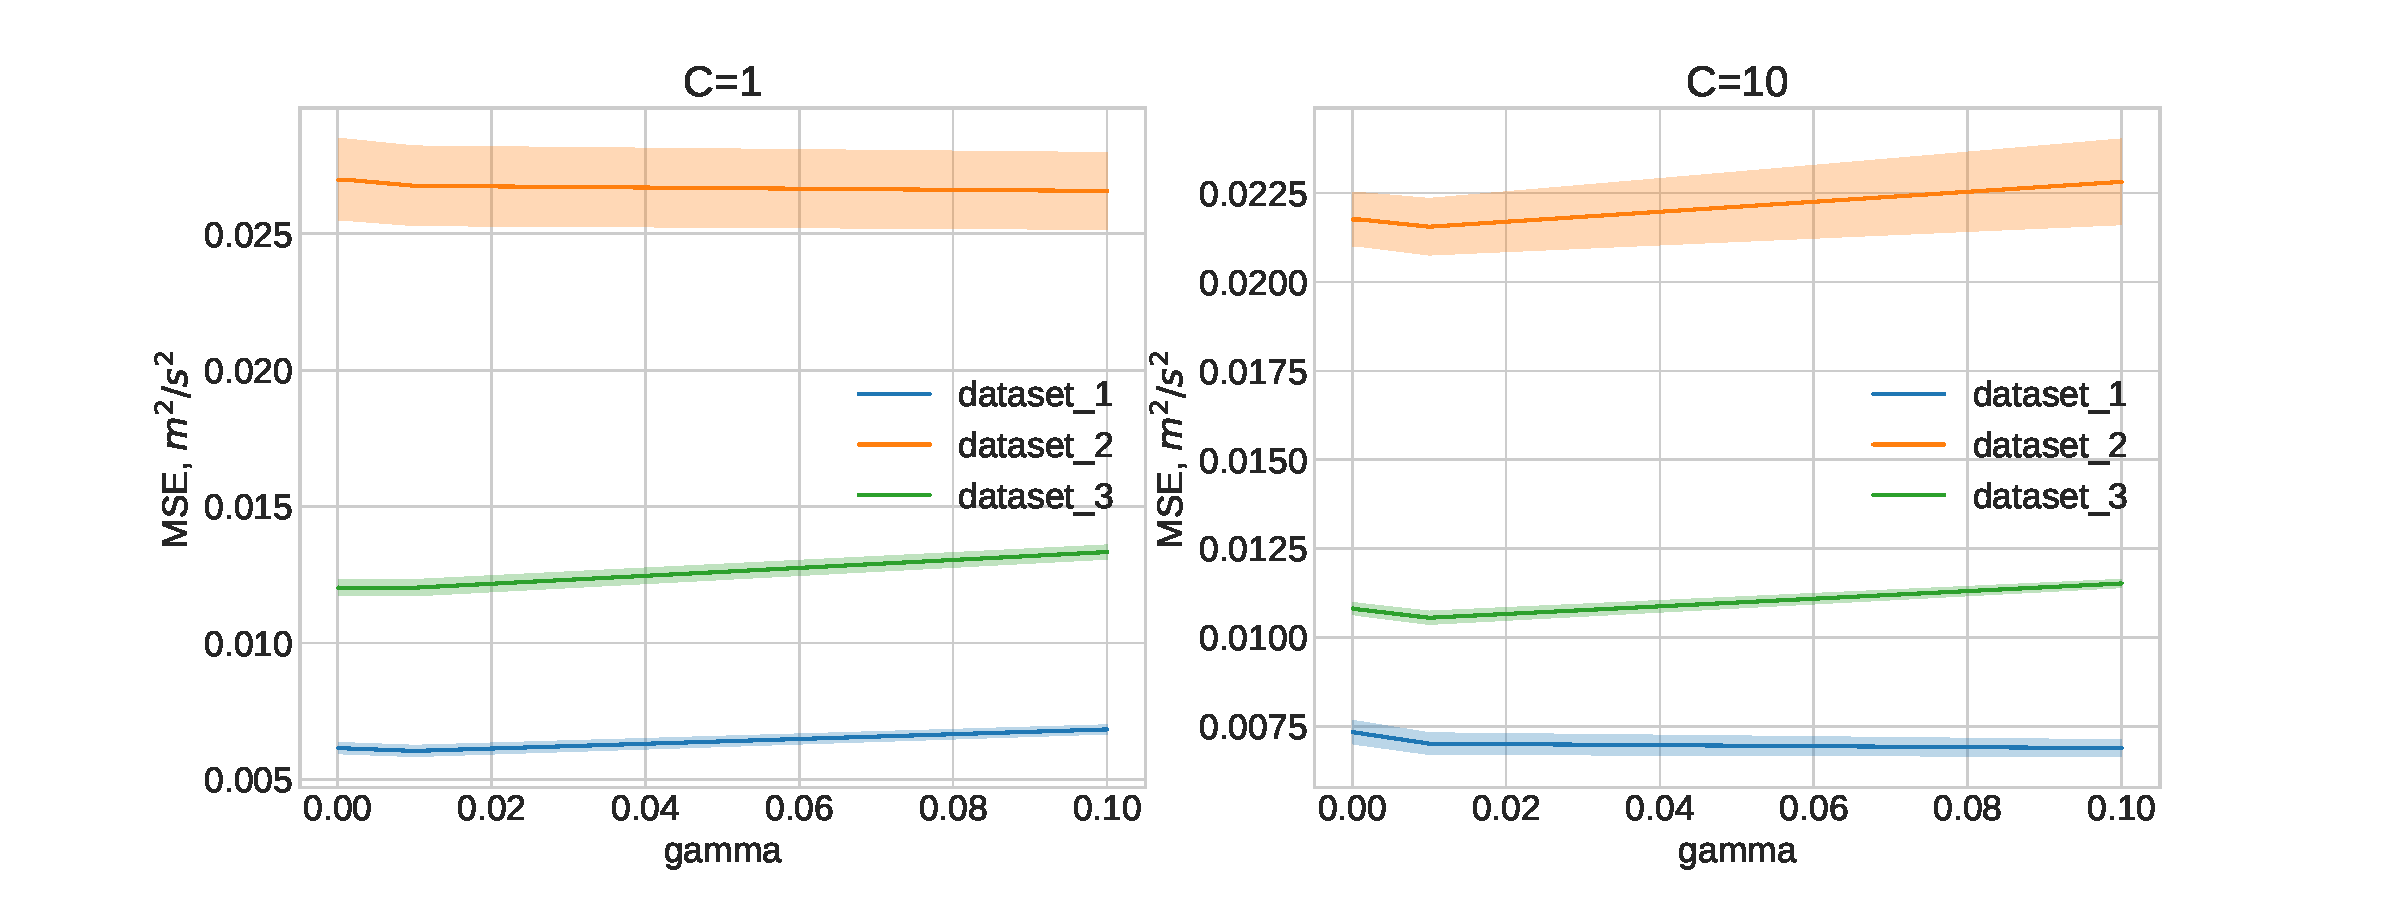
\includegraphics[scale=0.4]{charts/handheld_chn0_C=10.pdf}
    \caption{Рука, канал 0}
    \label{fig:image}
    \end{figure}
    
    \begin{figure}[H]
    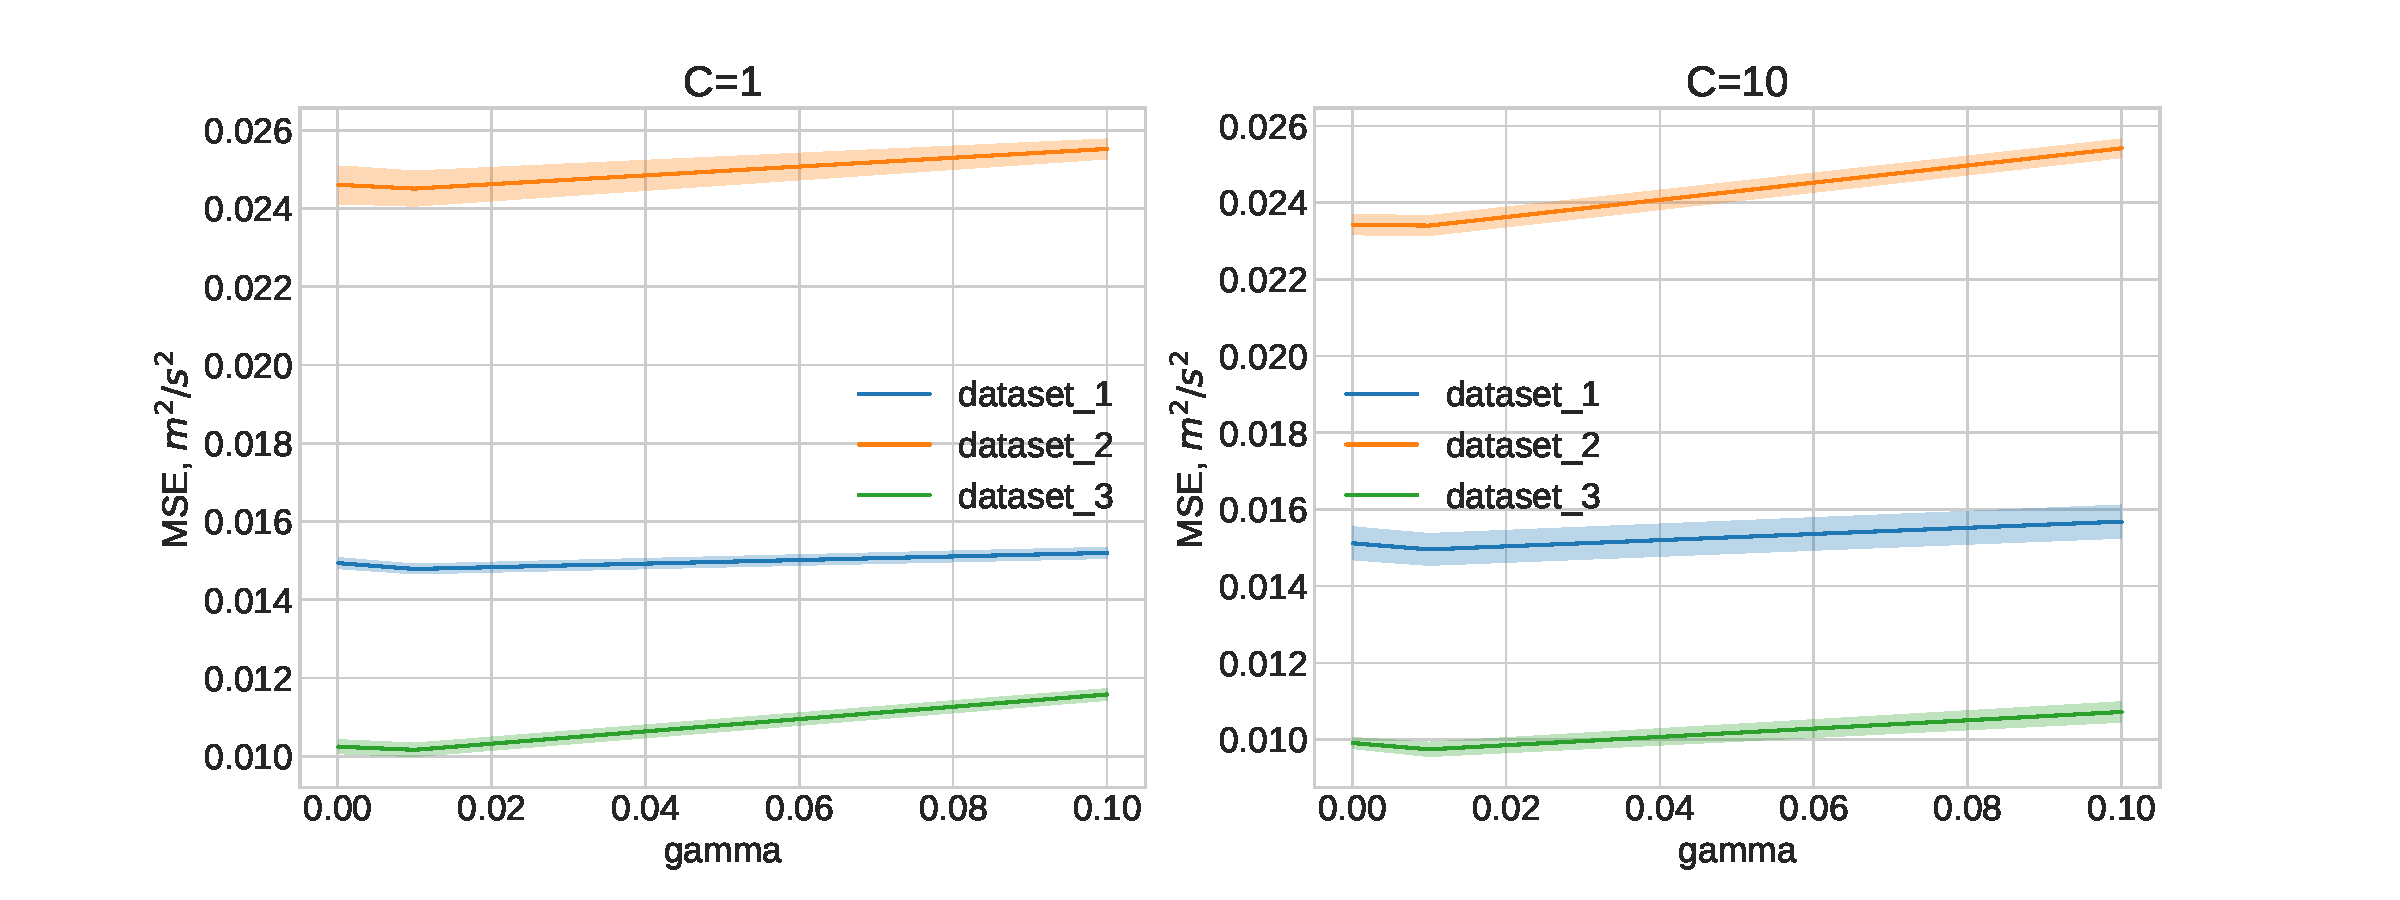
\includegraphics[scale=0.4]{charts/handheld_chn1_C=10.pdf}
    \caption{Рука, канал 1}
    \label{fig:image}
    \end{figure}
    
    \begin{figure}[H]
    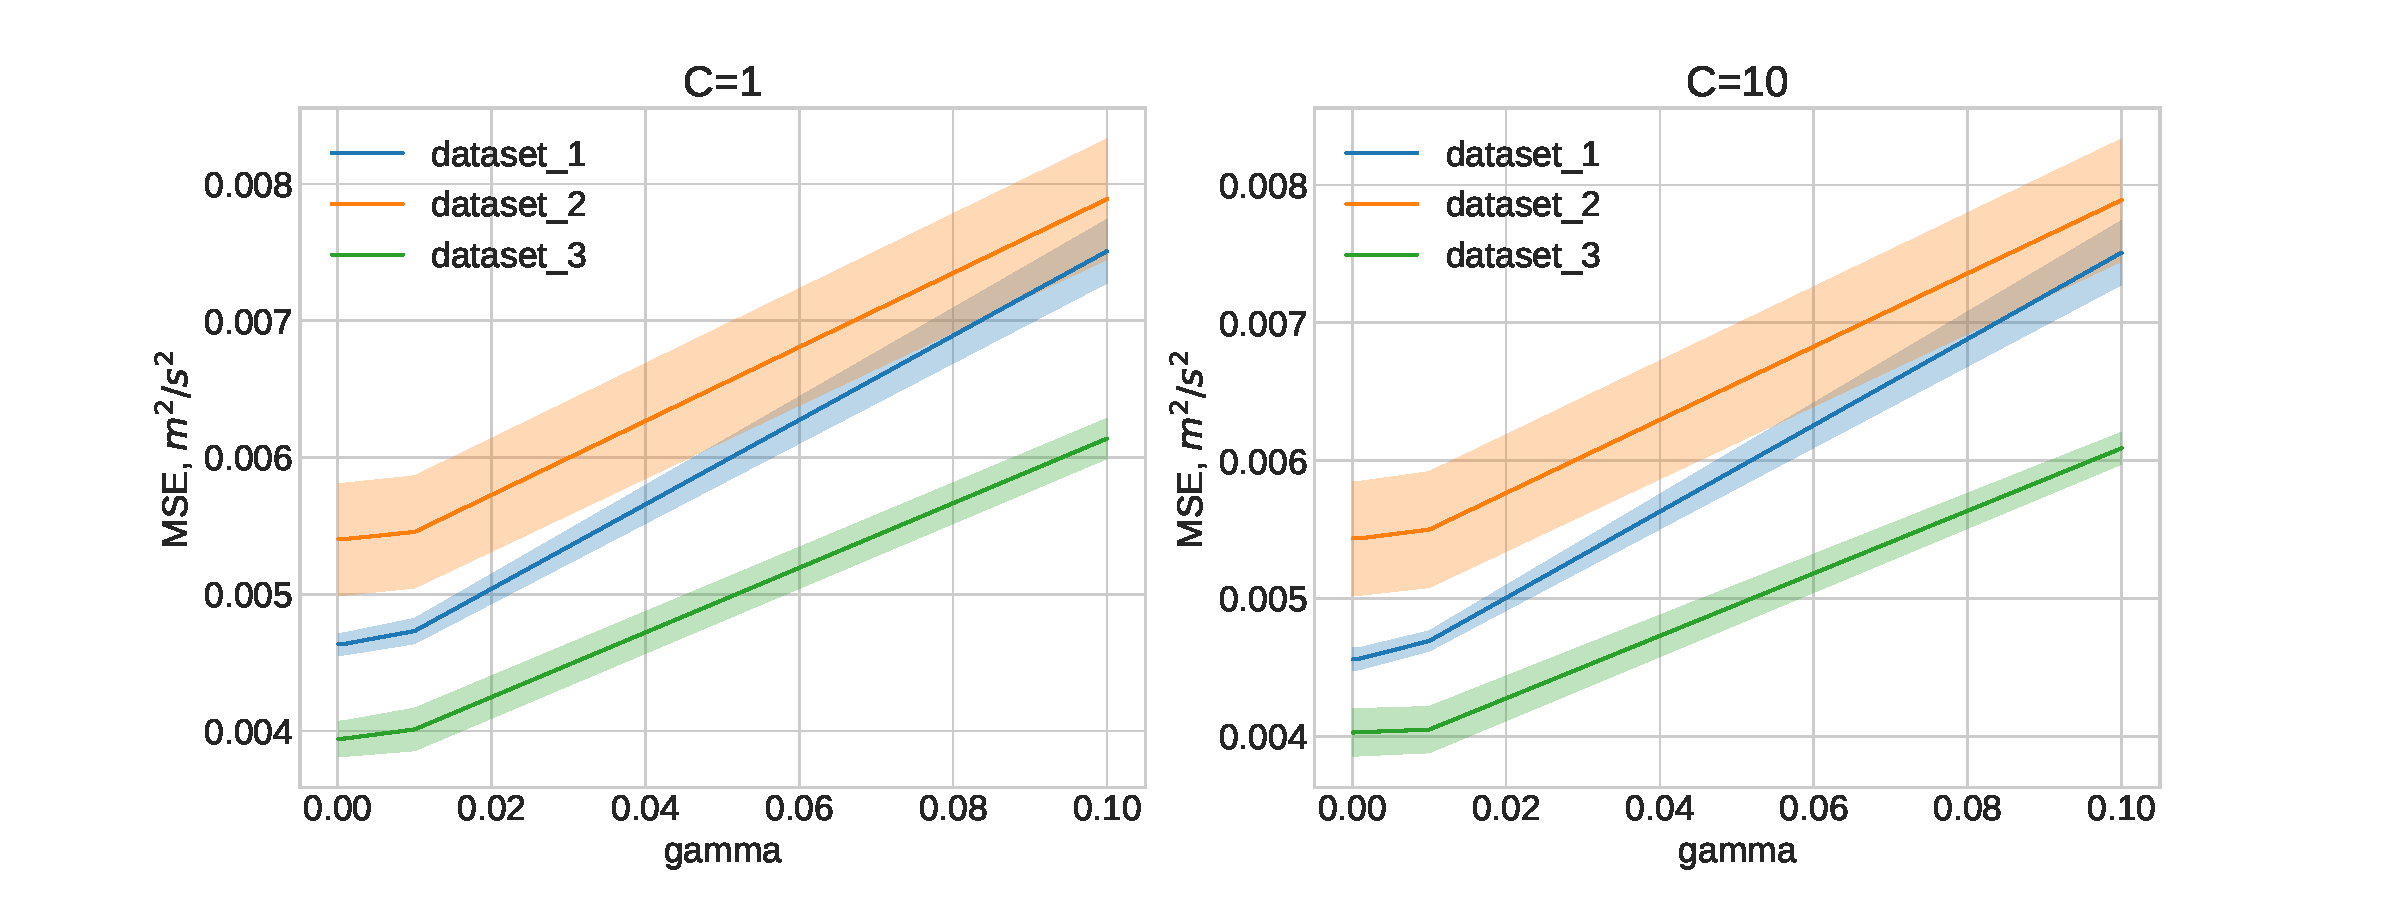
\includegraphics[scale=0.4]{charts/leg_chn0_C=10.pdf}
    \caption{Нога, канал 0}
    \label{fig:image}
    \end{figure}
    
    \begin{figure}[H]
    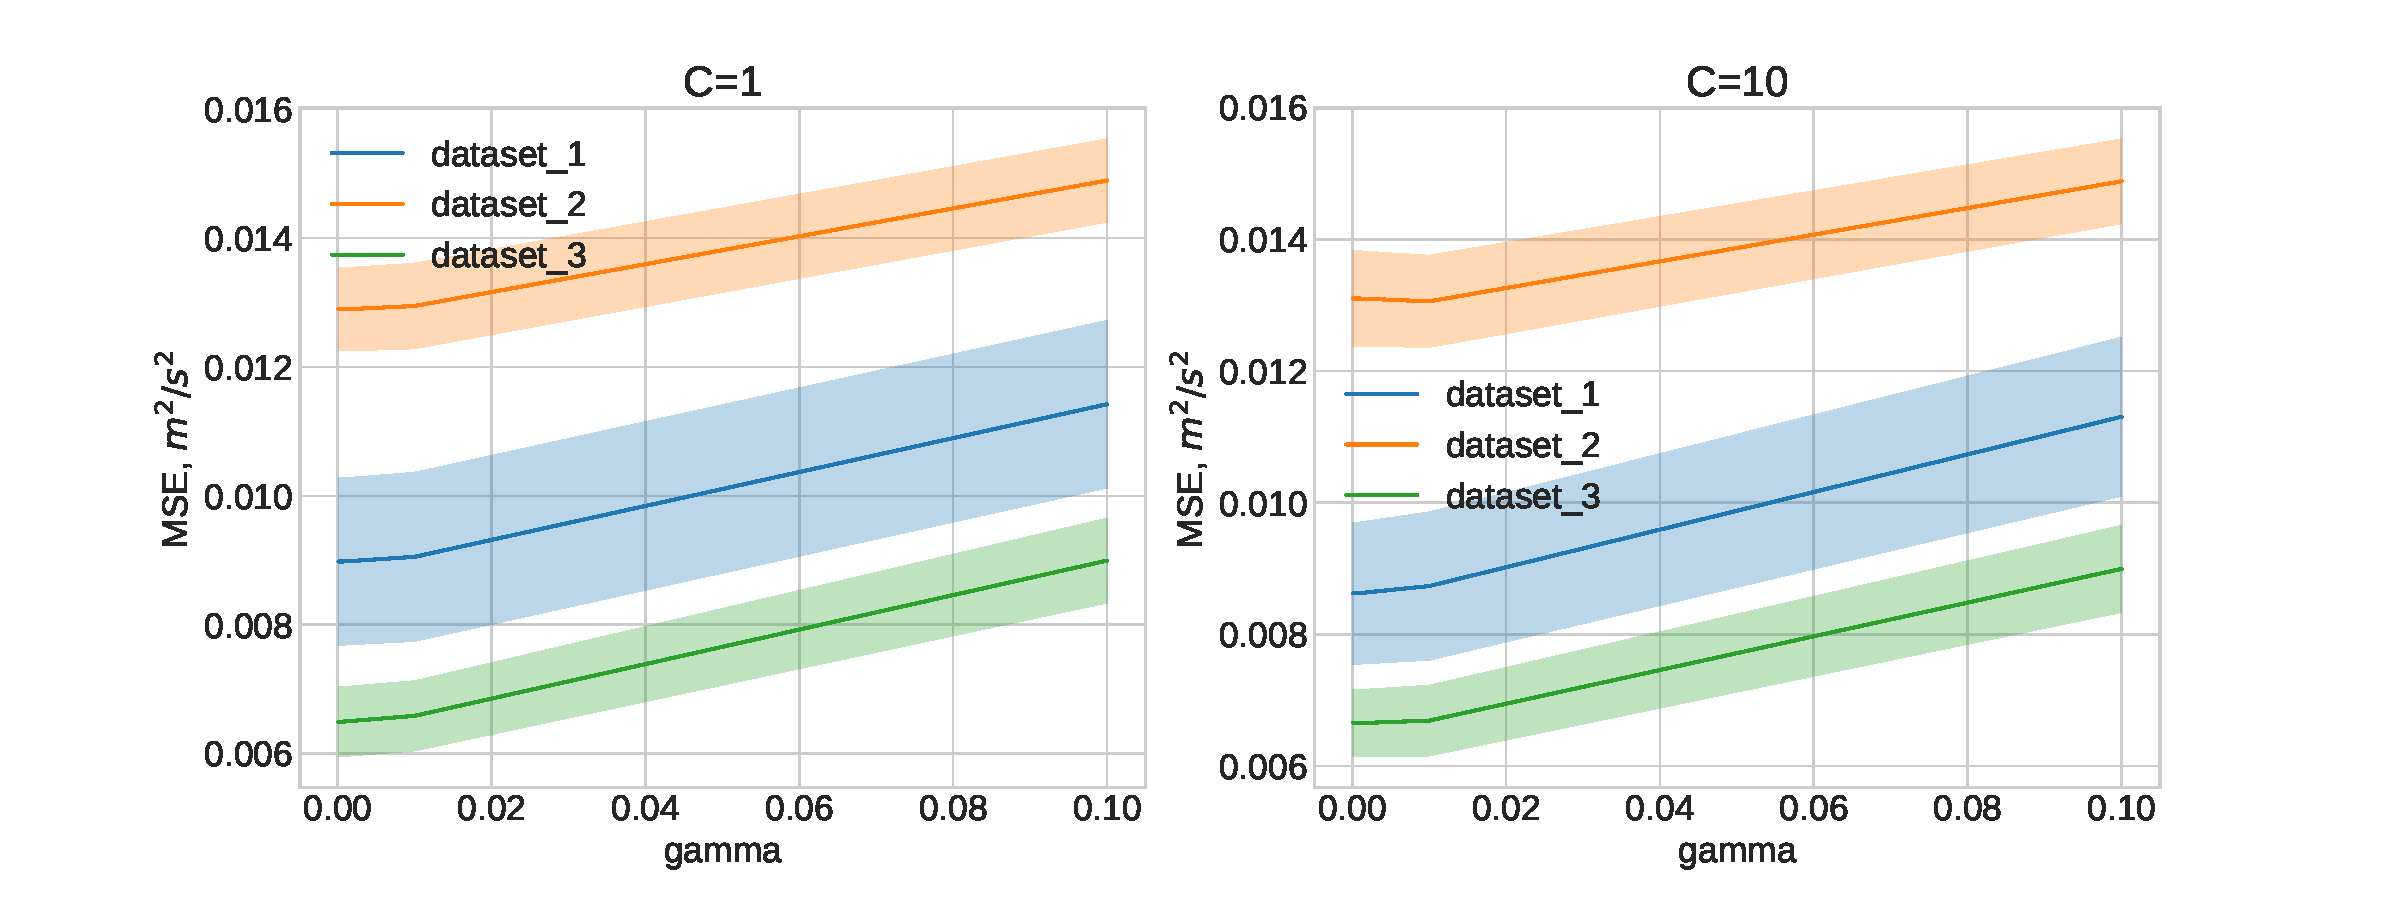
\includegraphics[scale=0.4]{charts/leg_chn1_C=10.pdf}
    \caption{Нога, канал 1}
    \label{fig:image}
    \end{figure}
    
    \begin{figure}[H]
    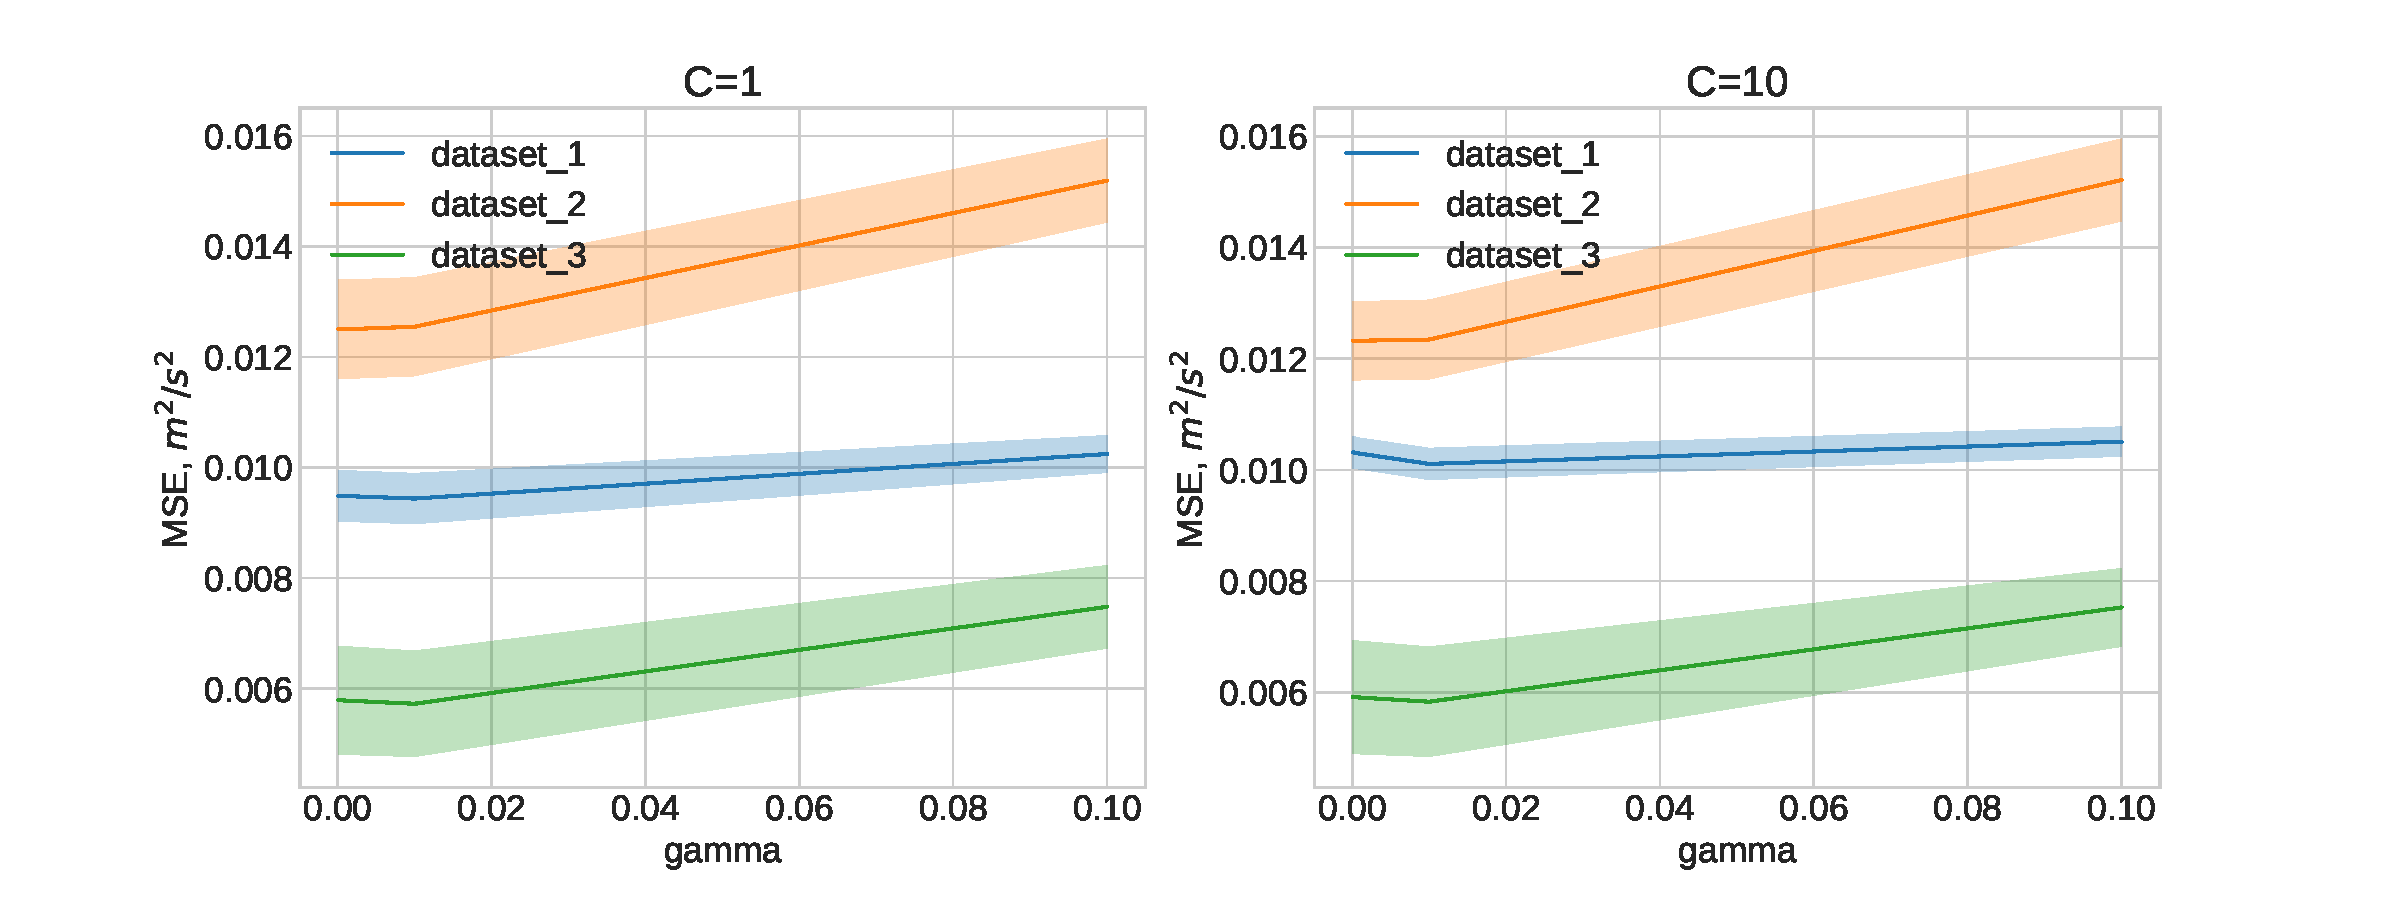
\includegraphics[scale=0.4]{charts/bag_chn0_C=10.pdf}
    \caption{Сумка, канал 0}
    \label{fig:image}
    \end{figure}
    
    \begin{figure}[H]
    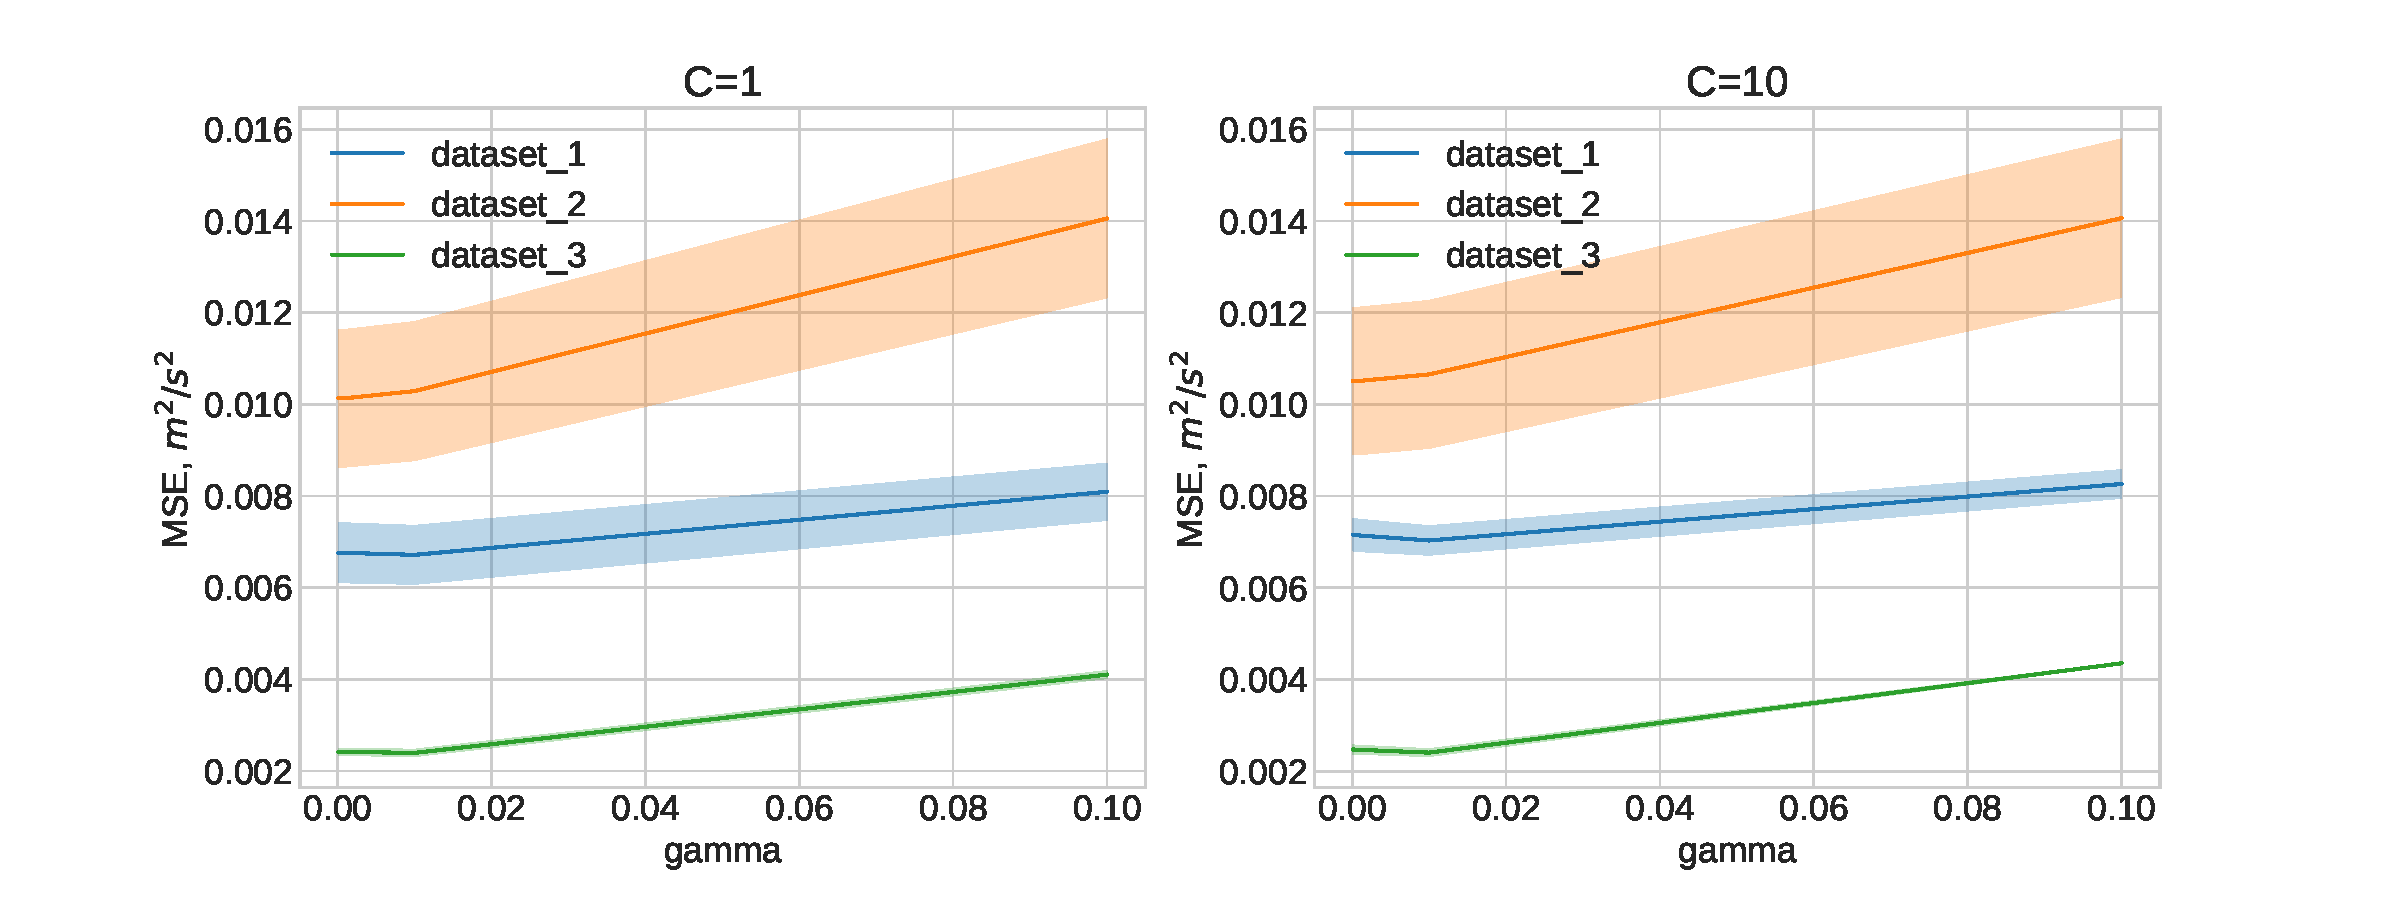
\includegraphics[scale=0.4]{charts/bag_chn1_C=10.pdf}
    \caption{Сумка, канал 1}
    \label{fig:image}
    \end{figure}
    
    \begin{figure}[H]
    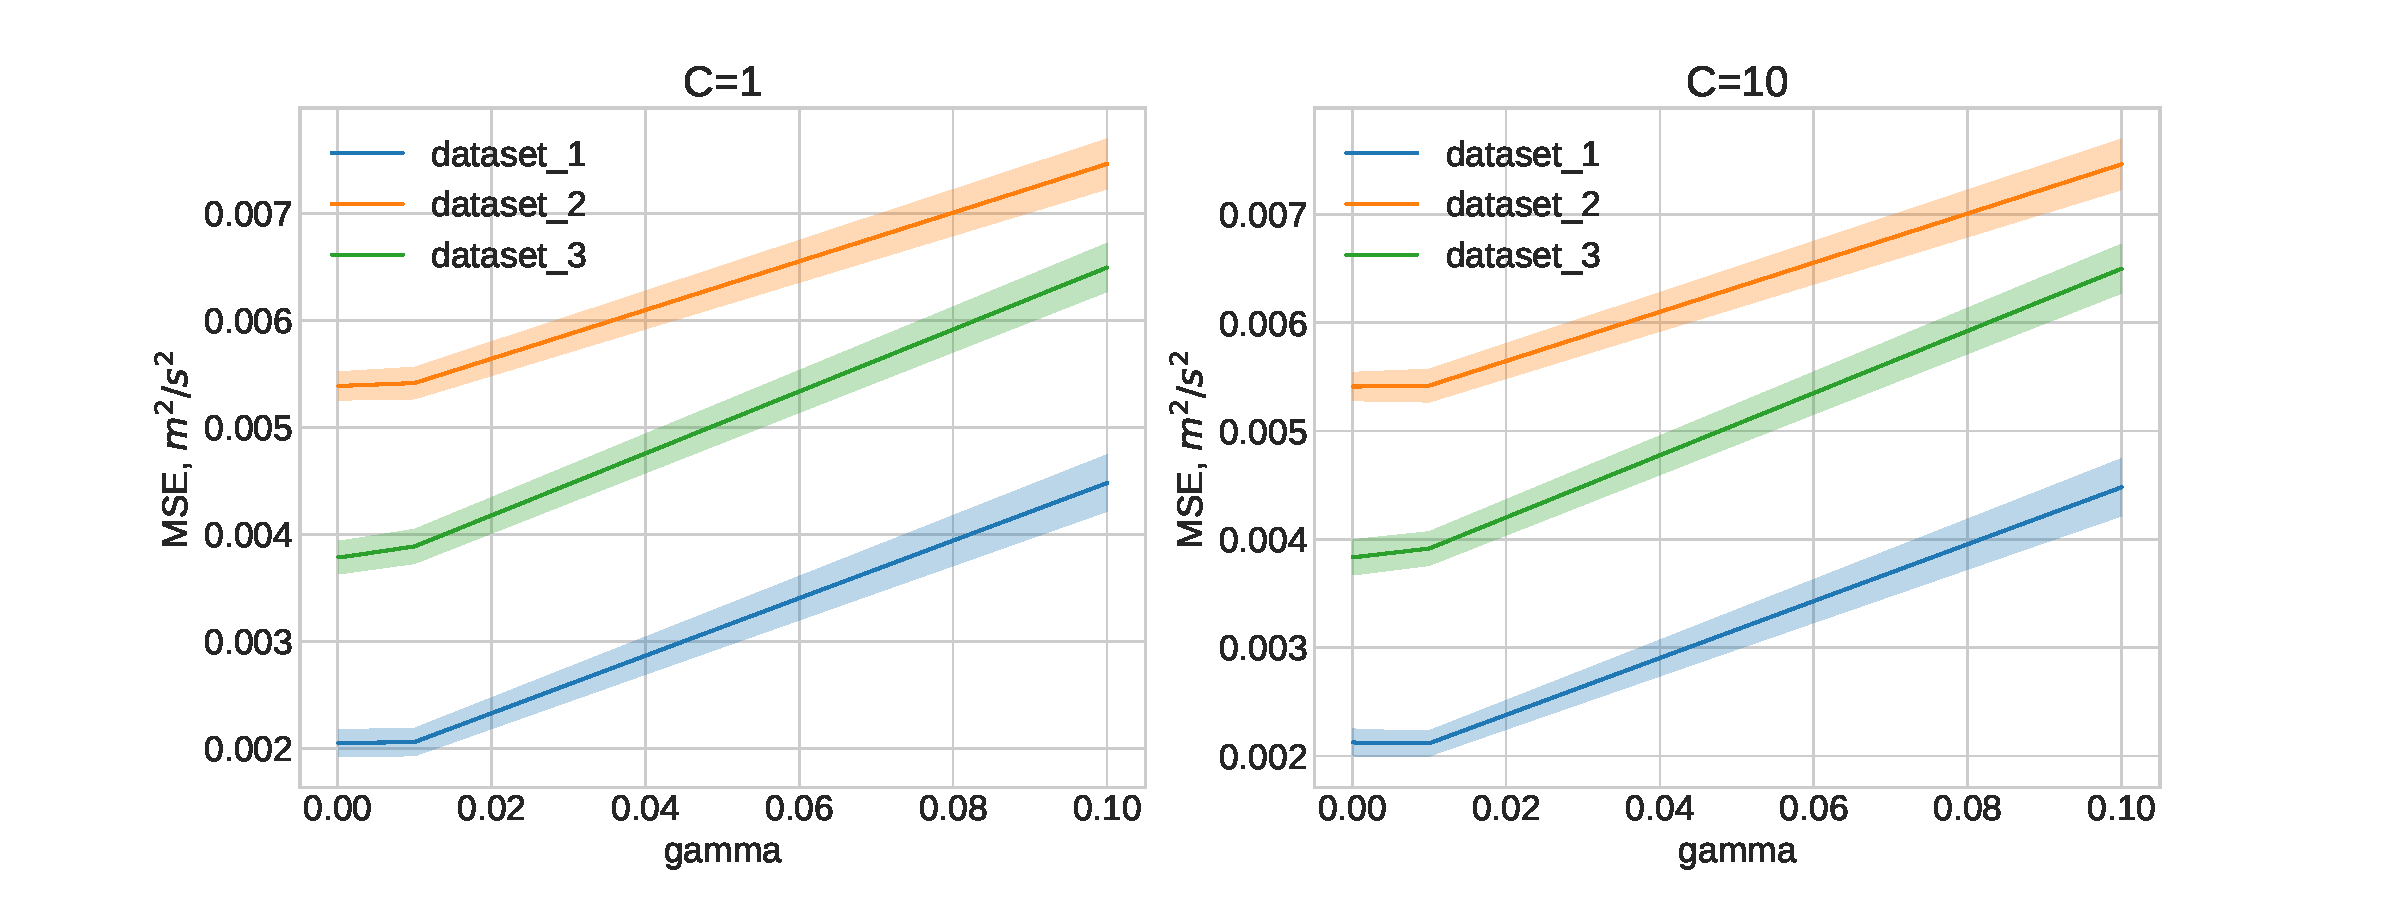
\includegraphics[scale=0.4]{charts/body_chn0_C=10.pdf}
    \caption{Тело, канал 0}
    \label{fig:image}
    \end{figure}
    
    \begin{figure}[H]
    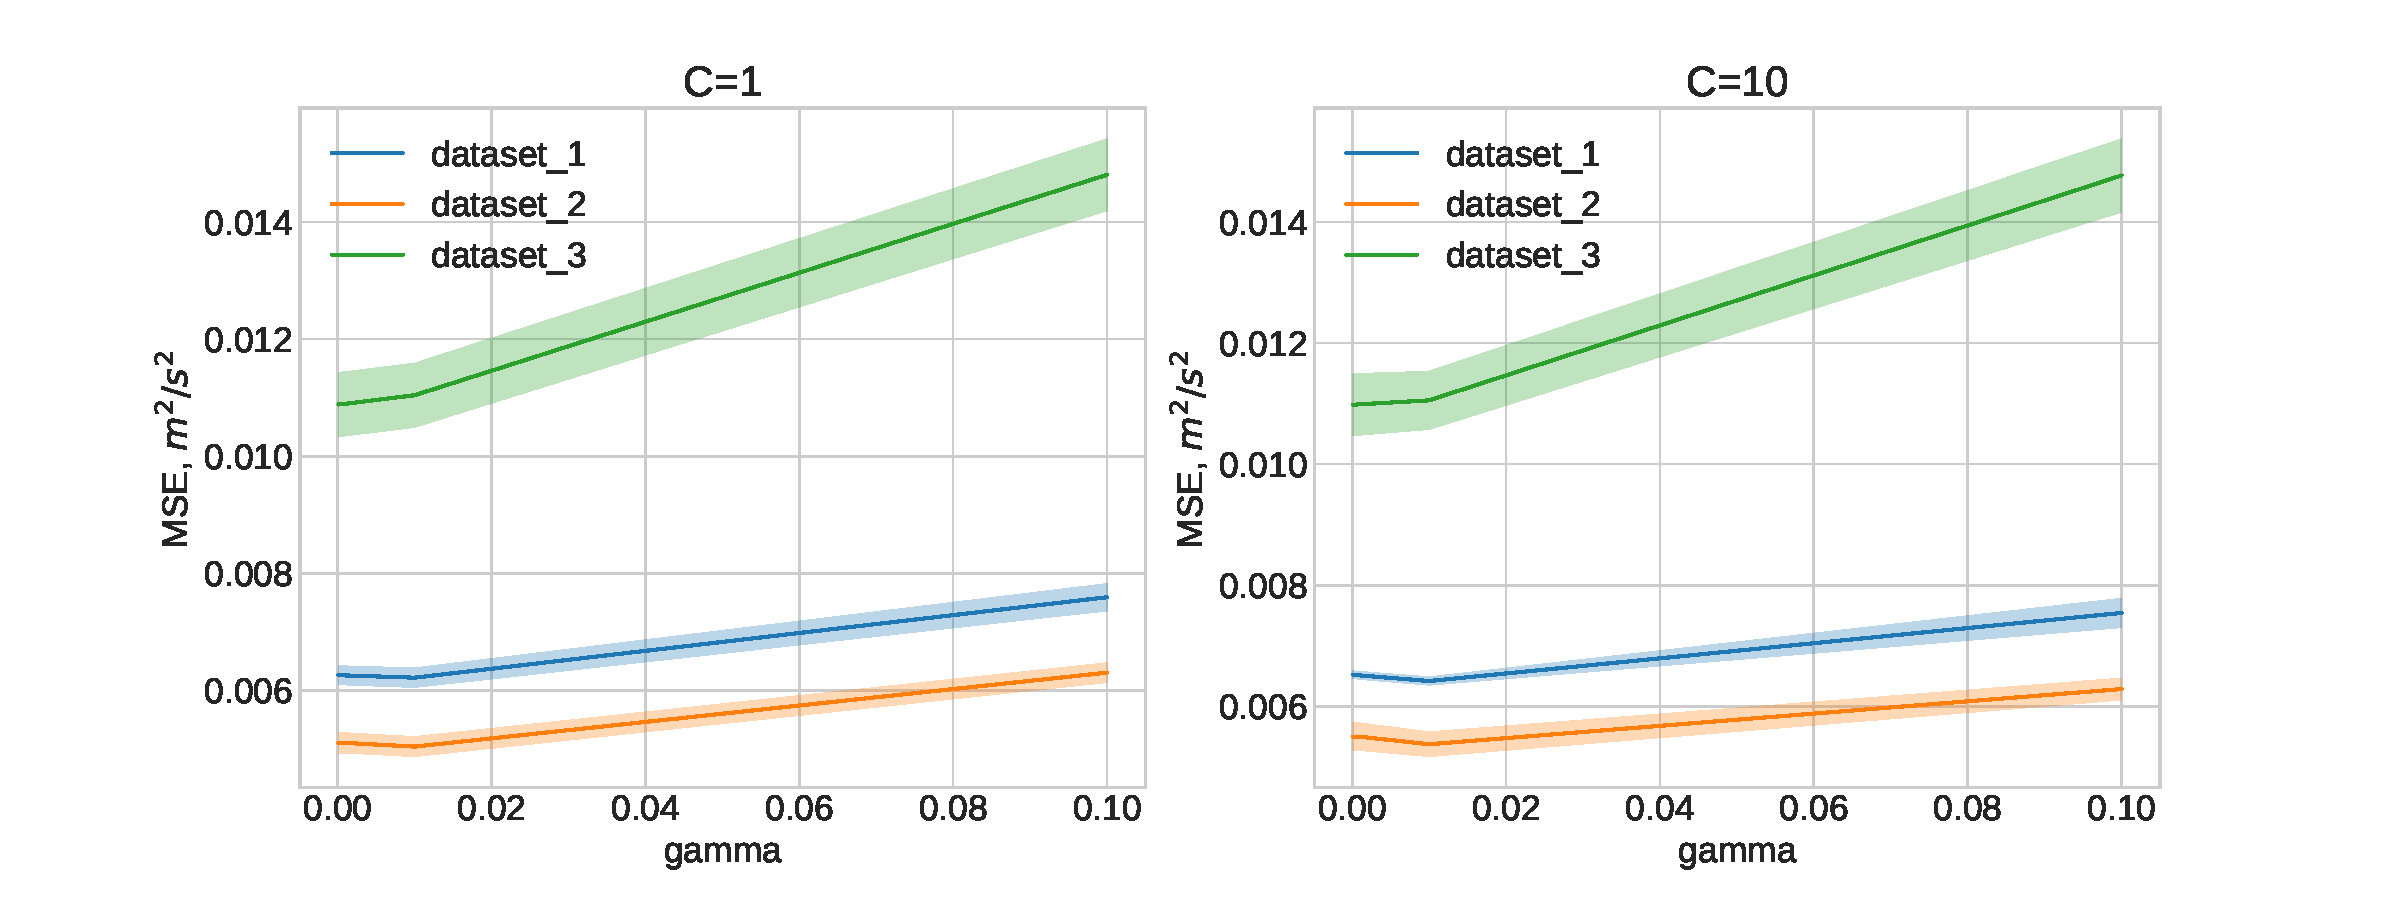
\includegraphics[scale=0.4]{charts/body_chn1_C=10.pdf}
    \caption{Тело, канал 1}
    \label{fig:image}
    \end{figure}
    
Для всех классов и выборок оптимальные значения параметра $\gamma$ близки к $0.001, 0.01$, поэтому при дальнейшем обучении моделей на большом количестве данных при заранее не заданных параметрах SVM-регрессоров, при поиске по сетке для параметра $\gamma$ будут использоваться только эти значения. Тогда для построенных моделей оптимальными параметрами будут следующие:

\begin{table}[H]
\begin{center}
\begin{tabular}{|c|c|c|c|c|}
\hline
& Рука & Нога & Сумка & Тело \\
\hline
C & 10 & 1 & 1 & 1 \\
\hline
$\gamma$ & 0.01 & 0.001 & 0.01 & 0.001\\
\hline
\end{tabular}
\end{center}
\end{table} 
    
По полученным значениям ошибок на кросс-валидации были выбраны оптимальные модели. С помощью этих моделей были построены траектории для каждого класса расположения смартфона (в качестве тестовой выборки была использована выборка Zhicheng). При этом траектории были построены для случаев, когда дополнительная корректировка весов с помощью оптимизации $V_{bias}$ не производилась (сиреневая линия) и когда производилась (синяя линяя). Истинная траектория обозначена красным цветом.

\begin{figure}[h]
\begin{minipage}[h]{0.49\linewidth}
\center{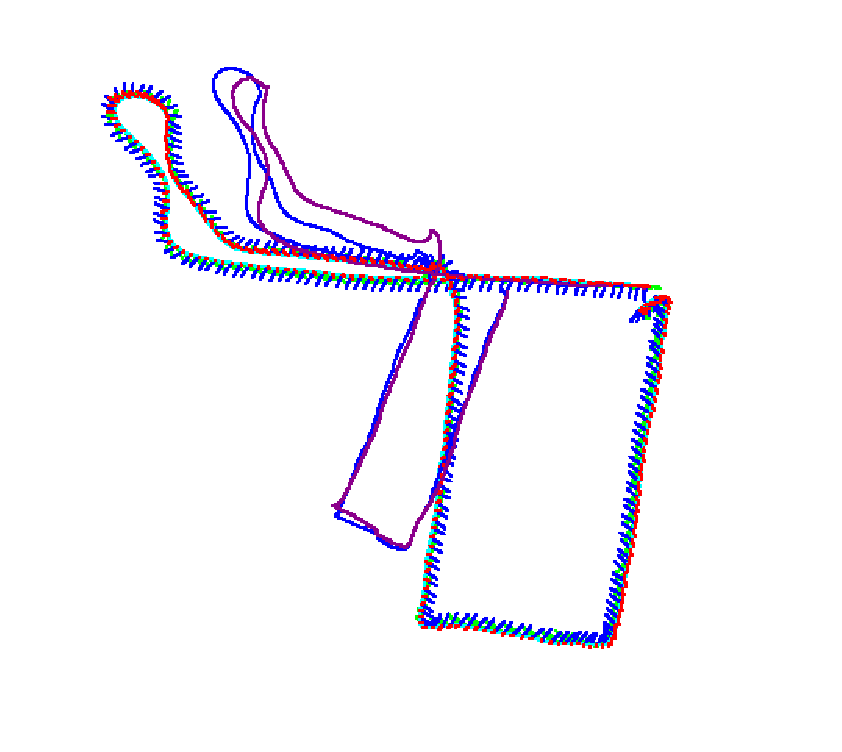
\includegraphics[width=0.5\linewidth]{trajectories/zhicheng_bag00.eps} \\ Класс-сумка}
\end{minipage}
\hfill
\begin{minipage}[h]{0.49\linewidth}
\center{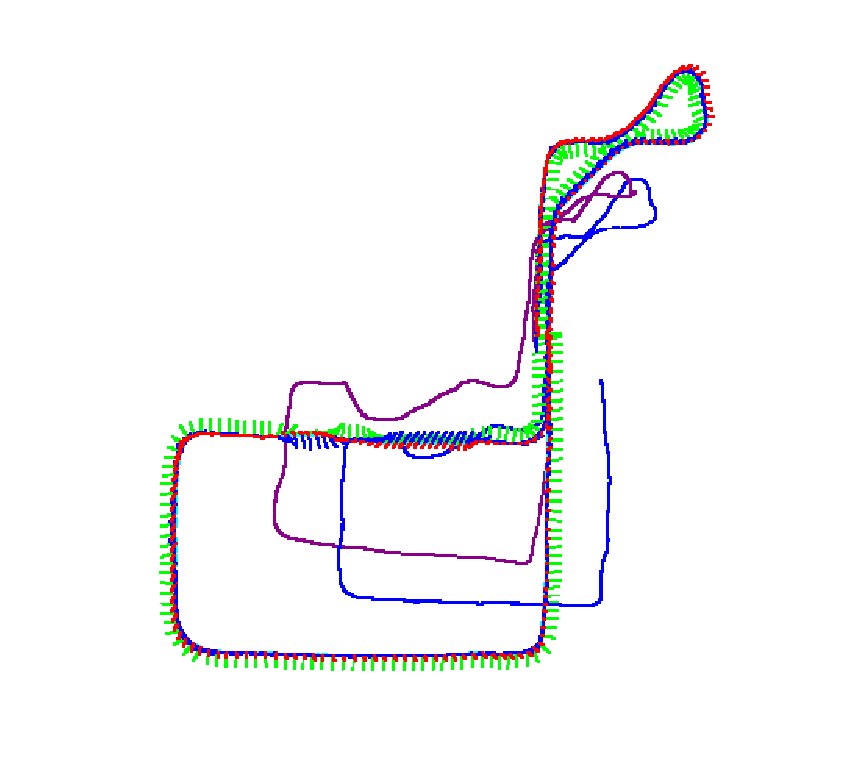
\includegraphics[width=0.5\linewidth]{trajectories/zhicheng_handheld00.eps} \\ Класс-рука}
\end{minipage}
\caption{Траектории}
\label{ris:image1}
\end{figure}

\begin{figure}[h]
\begin{minipage}[h]{0.49\linewidth}
\center{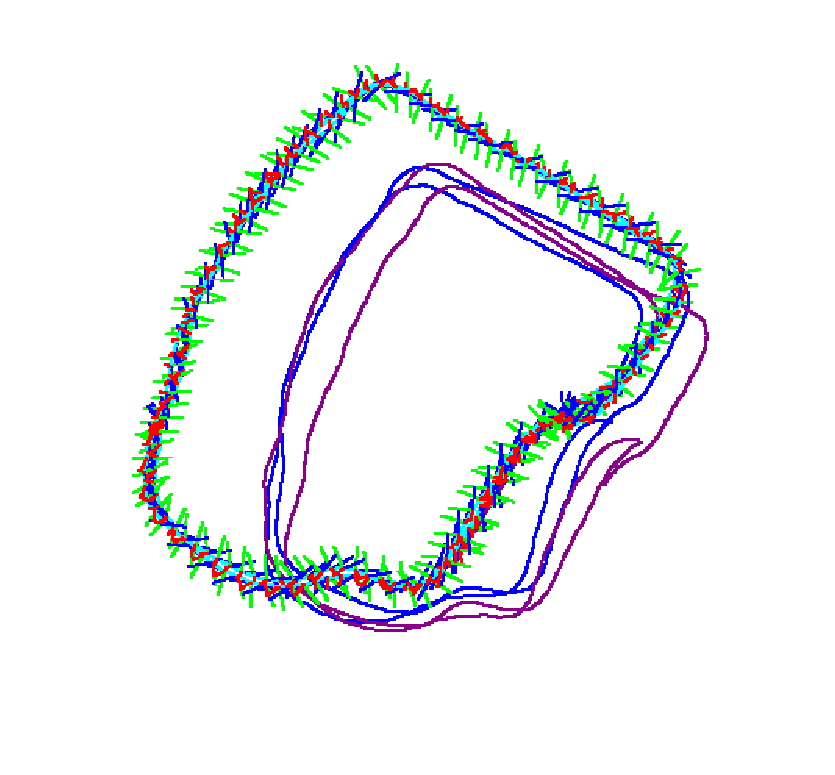
\includegraphics[width=0.5\linewidth]{trajectories/zhicheng_leg00.eps} \\ Класс-нога}
\end{minipage}
\hfill
\begin{minipage}[h]{0.49\linewidth}
\center{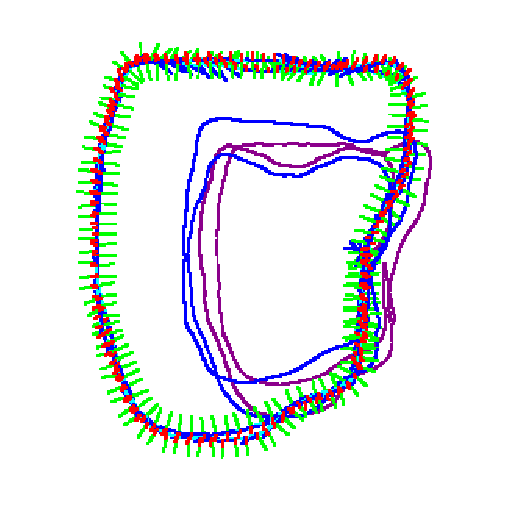
\includegraphics[width=0.5\linewidth]{trajectories/zhichenng_body00.eps} \\ Класс-тело}
\end{minipage}
\caption{Траектории}
\label{ris:image1}
\end{figure}

\section{Выводы}

Изначальное определение класса расположения смартфона помогло установить более подходящие параметры моделей, что увеличило точность предсказания. Также, как видно из рисунков полученных траекторий, дополнительное уточнение скоростей дает лучшее приближение истинных траекторий. В ходе данной работы были повторены результаты статьи RIDI~\cite{journals/corr/abs-1712-09004}. Также в этой статье при формировании выборки для уменьшения высокочастотного шума на изначальных данных предлагается применять фильтр Гаусса. В дальнейшем планируется применить полученную модель для дополнительно собранных данных, а также улучшить методы обработки данных для уменьшения шума (применение фильтра Калмана) и посмотреть другие способы оптимизации модели.


\newpage
\section{Приложения}
\rotatebox{90}{ %это обеспечивает поворот любого объекта
\begin{minipage}{1.5\linewidth}
\begin{table}[H]
\caption{Зависимости MSE ($m^2/s^2$) от параметров моделей для выборки 1}
\begin{center}
\begin{tabular}{|c|c|c|c|c|c|c|c|c|}
\hline
& \multicolumn{4}{c|}{C=1} & \multicolumn{4}{c|}{C=10} \\
\cline{2-9}
\raisebox{1.5ex}[0cm][0cm]{Регрессор}
& $\gamma=0.0001$ & $\gamma=0.001$ & $\gamma=0.01$ & $\gamma=0.1$
& $\gamma=0.0001$ & $\gamma=0.001$ & $\gamma=0.01$ & $\gamma=0.1$ \\
\hline
Сумка, 0
& $0.00949$ & $0.00948$ & $0.00944$ & $0.01025$
& $0.01032$
& $0.01029$
& $0.01011$
& $0.01051$ \\
\hline
Сумка, 1
& $0.00676$
& $0.00676$
& $0.00671$
& $0.00809$
& $0.00716$
& $0.00714$
& $0.00703$
& $0.00826$ \\
\hline
Тело, 0
& $0.00205$
& $0.00205$
& $0.00206$
& $0.00448$
& $0.00213$
& $0.00212$
& $0.00212$
& $0.00448$ \\
\hline
Тело, 1
& $0.00626$
& $0.00626$
& $0.00622$
& $0.00759$
& $0.00652$
& $0.00651$
& $0.00642$
& $0.00754$ \\
\hline
Рука, 0
& $0.00614$
& $0.00613$
& $0.00604$
& $0.00683$
& $0.00734$
& $0.00731$
& $0.00702$
& $0.00689$ \\
\hline
Рука, 1
& $0.01494$
& $0.01492$
& $0.01479$
& $0.0152$
& $0.01512$
& $0.0151$
& $0.01496$
& $0.01568$ \\
\hline
Нога, 0
& $0.00463$
& $0.00464$
& $0.00473$
& $0.00751$
& $0.00456$
& $0.00457$
& $0.00469$
& $0.00751$ \\
\hline
Нога, 1
& $0.00898$
& $0.00898$
& $0.00905$
& $0.01142$
& $0.00862$
& $0.00863$
& $0.00873$
& $0.01131$ \\
\hline

\end{tabular}
\end{center}
\end{table} 

\begin{table}[H]
\caption{Зависимости MSE ($m^2/s^2$) от параметров моделей для выборки 2}
\begin{center}
\begin{tabular}{|c|c|c|c|c|c|c|c|c|}
\hline
& \multicolumn{4}{c|}{C=1} & \multicolumn{4}{c|}{C=10} \\
\cline{2-9}
\raisebox{1.5ex}[0cm][0cm]{Регрессор}
& $\gamma=0.0001$ & $\gamma=0.001$ & $\gamma=0.01$ & $\gamma=0.1$
& $\gamma=0.0001$ & $\gamma=0.001$ & $\gamma=0.01$ & $\gamma=0.1$ \\
\hline
Сумка, 0
& $0.0125$
& $0.0125$
& $0.01255$
& $0.01519$
& $0.01232$
& $0.01232$
& $0.01234$
& $0.01521$\\
\hline
Сумка, 1
& $0.01013$
& $0.01013$
& $0.01029$
& $0.01406$
& $0.01051$
& $0.01051$
& $0.01065$
& $0.01406$ \\
\hline
Тело, 0
& $0.00205$
& $0.00205$
& $0.00206$
& $0.00448$
& $0.00213$
& $0.00212$
& $0.00212$
& $0.00448$ \\
\hline
Тело, 1
& $0.00511$
& $0.00511$
& $0.00504$
& $0.00631$
& $0.0055$
& $0.0055$
& $0.00537$
& $0.00629$ \\
\hline
Рука, 0
& $0.02699$
& $0.02699$
& $0.02676$
& $0.02657$
& $0.02176$
& $0.02176$
& $0.02155$
& $0.02282$ \\
\hline
Рука, 1
& $0.0246$
& $0.0246$
& $0.02451$
& $0.02552$
& $0.02342$
& $0.02342$
& $0.0234$
& $0.02541$ \\
\hline
Нога, 0
& $0.0054$
& $0.0054$
& $0.00546$
& $0.00789$
& $0.00544$
& $0.00544$
& $0.0055$
& $0.00789$ \\
\hline
Нога, 1
& $0.01289$
& $0.01289$
& $0.01295$
& $0.01489$
& $0.0131$
& $0.0131$
& $0.01306$
& $0.01488$ \\
\hline

\end{tabular}
\end{center}
\end{table} 
\end{minipage}
} 

\rotatebox{90}{ %это обеспечивает поворот любого объекта
\begin{minipage}{1.5\linewidth}
\begin{table}[H]
\caption{Зависимости MSE ($m^2/s^2$) от параметров моделей для выборки 3}
\begin{center}
\begin{tabular}{|c|c|c|c|c|c|c|c|c|}
\hline
& \multicolumn{4}{c|}{C=1} & \multicolumn{4}{c|}{C=10} \\
\cline{2-9}
\raisebox{1.5ex}[0cm][0cm]{Регрессор}
& $\gamma=0.0001$ & $\gamma=0.001$ & $\gamma=0.01$ & $\gamma=0.1$
& $\gamma=0.0001$ & $\gamma=0.001$ & $\gamma=0.01$ & $\gamma=0.1$ \\
\hline
Сумка, 0
& $0.00579$
& $0.00579$
& $0.00573$
& $0.00748$
& $0.00592$
& $0.00591$
& $0.00583$
& $0.00753$ \\
\hline
Сумка, 1
& $0.00242$
& $0.00241$
& $0.00239$
& $0.0041$
& $0.00247$
& $0.00247$
& $0.00241$
& $0.00435$ \\
\hline
Тело, 0
& $0.00379$
& $0.00379$
& $0.00389$
& $0.0065$
& $0.00384$
& $0.00384$
& $0.00391$
& $0.0065$ \\
\hline
Тело, 1
& $0.00511$
& $0.00511$
& $0.00504$
& $0.00631$
& $0.0055$
& $0.0055$
& $0.00537$
& $0.00629$ \\
\hline
Рука, 0
& $0.02699$
& $0.02699$
& $0.02676$
& $0.02657$
& $0.02176$
& $0.02176$
& $0.02155$
& $0.02282$ \\
\hline
Рука, 1
& $0.01025$
& $0.01024$
& $0.01016$
& $0.01158$
& $0.00991$
& $0.00989$
& $0.00975$
& $0.01072$ \\
\hline
Нога, 0
& $0.00394$
& $0.00395$
& $0.00401$
& $0.00614$
& $0.00403$
& $0.00403$
& $0.00405$
& $0.00609$ \\
\hline
Нога, 1
& $0.00649$
& $0.0065$
& $0.00659$
& $0.009$
& $0.00666$
& $0.00665$
& $0.00669$
& $0.00899$ \\
\hline

\end{tabular}
\end{center}
\end{table} 
\end{minipage}}









\bibliographystyle{plain}
\bibliography{Zainulina2018Project26}

\end{document}

